\documentclass{beamer}

% \usepackage{beamerthemesplit} // Activate for custom appearance

\mode<presentation>
{
  \usetheme{Darmstadt}      % or try Darmstadt, Madrid, Warsaw, ...
  \usecolortheme{default} % or try albatross, beaver, crane, ...
  \usefonttheme{default}  % or try serif, structurebold, ...
  \setbeamertemplate{navigation symbols}{}
  \setbeamertemplate{caption}[numbered]
}

\title{Probability Basics}
\author{Cameron Beebe}
\institute
{
The SciPhi Initiative, LLC
\medskip
}
\date{\today}
\newcommand{\indep}{\perp \!\!\! \perp}
\usepackage{graphicx}
\usepackage{amssymb}
\usepackage{tikz}
\usetikzlibrary{bayesnet}
\usetikzlibrary{arrows, decorations.markings, matrix, decorations.pathmorphing}
\usetikzlibrary{decorations.pathreplacing}
\usepackage{pgfplots}
\usepackage{pgfplotstable}
\pgfplotsset{compat=newest}
%\usepgfplotslibrary{clickable}
\usetikzlibrary{shapes}
\usetikzlibrary{plotmarks}
\usepackage{relsize}
\usepackage{natbib}
\usepackage{bussproofs}
\usepackage{hyperref}
\hypersetup{
    colorlinks=true,
    linkcolor=blue,
    filecolor=magenta,      
    urlcolor=cyan,
}
\sloppy

\begin{document}

\frame{\titlepage}

\section[Outline]{}
\frame{\tableofcontents}

\section{Kolmogorov Axioms}
\frame
{
\frametitle{Kolmogorov Axioms}

\begin{itemize}
    \item<1->  Probabilities are defined by a probability measure $P$ over a space (universe) $\Omega$ of events $E_i$.  
    \begin{enumerate}
    \item<2->  $P(E_i) \geq 0$  for any $E_i \in \Omega$
    \item<3->  $P(\Omega) = 1$ 
    \begin{itemize} 
    \item<4-> (...which is equal to the probability of the disjoint union $P(\bigsqcup T_j)$ for $T_j$ partitions of $\Omega$, i.e. $\Omega = \bigsqcup T_j$)
    \end{itemize}
    \item<5->  $P(E_1 \lor E_2 \lor ...) = \Sigma_i P(E_i)$ for $E_i \cap E_{j\neq i} = \{\}$ for each $i,j$
    \item<6->  NOTE: Notation and terminology can vary.  E.g. conjunctions of events (joint probabilities) might be represented by $\cap$, $\land$, $\&$, or commas.  
    \end{enumerate}
\end{itemize}



}

\frame
{
\frametitle{Venn Diagram Representations}
\begin{center}
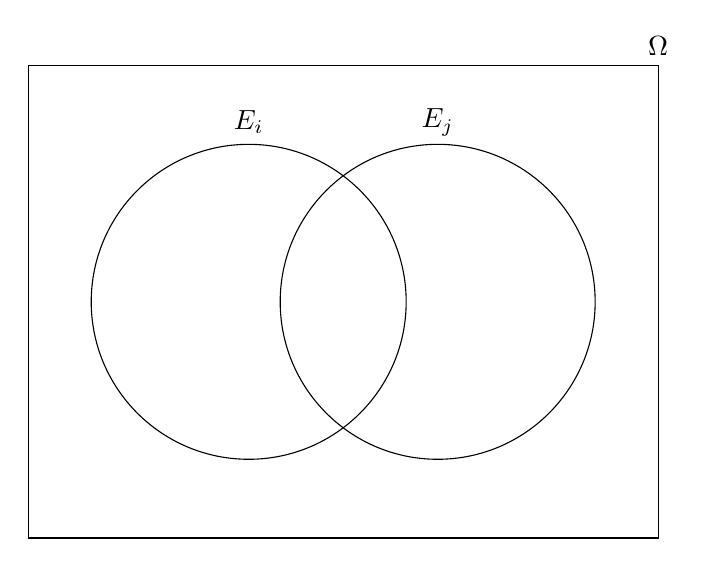
\begin{tikzpicture}[
dot/.style = {circle, inner sep=0pt, minimum size=1mm, fill,
              node contents={}}
                        ]
\def\firstcircle{(-1.2,0) coordinate (a) circle (2cm)}
\def\secondcircle{(1.2,0) coordinate (b)  circle (2cm)}
%\begin{scope}
%\clip (-2,-2) rectangle (2,2)
%\clip \secondcircle;
%\fill[cyan] \firstcircle;
%\end{scope}
\draw \firstcircle;
\draw \secondcircle;
\node (c) [above] at (current bounding box.north -| a) {$E_i$};
\node at (c -| b) {$E_j$};
\draw (-4,-3) rectangle (4,3) node [text=black,above] {$\Omega$};
\end{tikzpicture}
\end{center}
}


\frame
{
\frametitle{A Few More Definitions}

\begin{itemize}
    \item<1-> Conditional Probability: $P(A|B) = \frac{P(A\cap B)}{P(B)}$
    \item<2-> Independence: $P(A\cap B) = P(A)P(B)$ implies $A\indep B$
    \item<3-> Screening Off: $P(A|B\cap C) = P(A|B)$ implies $A\indep C$.  
    \item<4-> Bayes' Theorem:  $P(A|B) = \frac{P(B|A)P(A)}{P(B)}$, $P(B) \neq 0$
\end{itemize}

}


\frame{
\frametitle{Proof of Bayes' Theorem}

\begin{itemize}
    \item<1-> $P(A|B)P(B) = P(A\cap B) $
    \item<2-> $P(B|A)P(A) = P(B \cap A)$
    \item<3->  By commutativity of the set intersection, we can see that $P(A|B)P(B) = P(B|A)P(A)$
    \item<4-> Then substitute into definition of conditional probability.
    \item<5-> $P(A|B) = \frac{P(B|A)P(A)}{P(B)}$ 
\end{itemize}



}




\section{Frequency Interpretation}
\frame
{
\frametitle{Law of Large Numbers}

\begin{itemize}
    \item<1->  The probability of $E$ is determined by the frequency of occurrence in a statistical manner.  $P_f(E)$
    \item<2->  Or, a limiting ratio as more samples are observed. (Fisher)
\end{itemize}

}

\frame
{
\frametitle{Fisher Quote}

\begin{quote}
    To such a [man gambling on a single die throw] the information supplied by a familiar mathematical statement such as: ``If $a$ aces are thrown in $n$ trials, the probability that the difference in absolute value between $a/n$ and $1/6$ shall exceed any positive value $\epsilon$, however small, shall tend to zero as the number $n$ is increased indefinitely'', will seem not merely remote, but also incomplete and lacking in definiteness in its application to the particular throw in which he is interested.  Indeed, by itself it says nothing about that throw.  It is obvious, moreover, that many subsets of future throws, which may include his own, can be shown to give probabilities, in this sense, either greater or less than $1/6$.  
\end{quote}



}

%\section{Frequency v. Propensity}









\section{Subjective Degrees of Belief}
\frame
{
\frametitle{Bayesian Dutch Book}

\begin{itemize}
    \item<1->  Probabilities are (Subjective) Degrees of Belief $P_b$.
    \item<2->  Coherence:  Degrees of Belief should obey axioms of probability
    \begin{itemize}
        \item<3-> e.g. $\Sigma_i P_b(E_i) = 1$ for all $E_i \in \Omega_b$ 
        \item<4-> e.g. $P_b(E_i) \geq 0$ for all $E_i \in \Omega_b$
        \item<5-> e.g. $P_b(E_i \lor E_j)$ should equal $P_b(E_i) + P_b(E_j)$ for disjoint $E_i,E_j \in \Omega_b$ 
    \end{itemize}
    \item<6->  If one is Incoherent (i.e. violates axioms of probability) in subjective degrees of belief, it would be possible for a ``Dutch Bookie'' to construct a list of bets (which you would take!) such that a loss is certain.  
    \item<7-> Consider belief that a fair $n$-sided object has $P_b(E) \neq \frac{1}{n}$.
    \item<8-> Price: $Pr(E) := $ price an agent willing to pay for a ticket that pays 1 in the case that $E$ occurs, and 0 otherwise.
\end{itemize}

}



%\subsection{Proper Scoring (de Finetti)}

\frame
{
\frametitle{Proper Scoring}

\begin{itemize}
    \item<1-> de Finetti actually saw problems with Dutch Book and betting definitions, as the DoB they elicit might be unduly influenced by other parties.
    \begin{itemize}
        \item<2-> Betting ``on the open market,'' where there is some interaction between the Bookie and the agent could bias elicitation (and calibration).
    \end{itemize}
    \item<3-> Instead, he preferred what is called proper scoring rules.
    \begin{itemize}
        \item<4->  Belief calibration should occur against one's own lights: it is not fundamentally about what you can win on the open market, but about not losing what you already have.
    \end{itemize}
    
\end{itemize}

}


\frame
{
\frametitle{Proper Scoring}

An individual is asked to provide their DoB or subjective estimation \math \pi \endmath\space of an event \math E \endmath, with the knowledge that he or she will be scored according to whether \math E \endmath\space obtains or not---and whether \math \pi \endmath\space corresponds with their actual degree of belief \math p \endmath.  A penalization is calculated using the quadratic formula \math (E - \pi)^2 \endmath, where \math E \endmath\space is 1 or 0.  The prevision or expectation of this penalization is \math (E - \pi)^2(1 - p) + (E^c - \pi)^2(p) \endmath, or the sum of the assessments in the case that \math E \endmath\space obtains or does not obtain (\math E^c \endmath).  When \math E = 1 \endmath\space (and \math E^c = 0 \endmath) this simplifies to \math \pi^2 + p - 2\pi{p} \endmath.    In the case that one does not state one's \textit{actual} degree of belief (\math \pi \neq p \endmath), the prevision of penalization increases by \math (\pi - p)^2 \endmath.    This algebraic fact is the basis of why proper scores are seen to be an effective elicitor of subjective DOB.

%\cite[p. 16, 27-28]{deFinetti2008}
%\cite[p. 16]{deFinetti2008}
}


\frame
{
\frametitle{Principal Principle (Lewis)}

\begin{itemize}
    \item<1-> Subjective Degrees of Belief should respect observed frequencies. 
    \item<2-> That is, $P_b(E)$ should equal $P_f(E)$
\end{itemize}


}


\frame
{
\frametitle{Propensities (Popper)}

\begin{itemize}
    \item<1->  Probabilities are propensities or dispositions of systems to exhibit certain frequencies. 
    \item<2->  Objective vs. Subjective
\end{itemize}

}



\end{document}